\documentclass{article}
%%%%%%%%%%%%%%%%%%%%%%%%%%%%%%%%%%%%%%%%%%%%%%%%%%%%%%%%%%%%%%%%%%%%%%%%%%%%%%%%%%%%%%%%%%%%%%%%%%%%%%%%%
\usepackage{csquotes,xpatch}% recommended
\usepackage[backend=bibtex,
style=authoryear-comp,
sortcites=false,
maxbibnames=5,maxcitenames=2,
firstinits=true,
natbib=true,
]{biblatex}

\addbibresource{refs.bib}

% natbib = true: add comma between author and year
% firstinits: for first name initials in bibliography
\renewcommand{\postnotedelim}{ } % remove comma in post citation in autocite
%\addbibresource{refs.bib}
%%%%%%%%%%%%%%%%%%%%%%%%%%%%%%%%%%%%%%%%%%%%%%%%%%%%%%%%%%%%%%%%%%%%%%%%%%%%%%%%%%%%%%%%%%%%%%%%%%%%%%%%%

% Combine label and labelyear links
\xpatchbibmacro{cite}
{\usebibmacro{cite:label}%
	\setunit{\addspace}%
	\usebibmacro{cite:labelyear+extrayear}}
{\printtext[bibhyperref]{%
		\DeclareFieldAlias{bibhyperref}{default}%
		\usebibmacro{cite:label}%
		\setunit{\addspace}%
		\usebibmacro{cite:labelyear+extrayear}}}{}{}

% Include labelname in labelyear link
\xpatchbibmacro{cite}
{\printnames{labelname}%
	\setunit{\nameyeardelim}%
	\usebibmacro{cite:labelyear+extrayear}}
{\printtext[bibhyperref]{%
		\DeclareFieldAlias{bibhyperref}{default}%
		\printnames{labelname}%
		\setunit{\nameyeardelim}%
		\usebibmacro{cite:labelyear+extrayear}}}{}{}

% Access hyperref's citation link start/end commands
\makeatletter
\protected\def\blx@imc@biblinkstart{%
	\@ifnextchar[%]
	{\blx@biblinkstart}
	{\blx@biblinkstart[\abx@field@entrykey]}}
\def\blx@biblinkstart[#1]{%
	\blx@sfsave\hyper@natlinkstart{\the\c@refsection @#1}\blx@sfrest}
\protected\def\blx@imc@biblinkend{%
	\blx@sfsave\hyper@natlinkend\blx@sfrest}
\blx@regimcs{\biblinkstart \biblinkend}
\makeatother

\newbool{cbx:link}

% Include parentheses around labelyear in \textcite only in
% single citations without pre- and postnotes
\def\iflinkparens{%
	\ifboolexpr{ test {\ifnumequal{\value{multicitetotal}}{0}} and
		test {\ifnumequal{\value{citetotal}}{1}} and
		test {\iffieldundef{prenote}} and
		test {\iffieldundef{postnote}} }}

\xpatchbibmacro{textcite}
{\printnames{labelname}}
{\iflinkparens
	{\DeclareFieldAlias{bibhyperref}{default}%
		\global\booltrue{cbx:link}\biblinkstart%
		\printnames{labelname}}
	{\printtext[bibhyperref]{\printnames{labelname}}}}{}{}

\xpatchbibmacro{textcite}
{\usebibmacro{cite:label}}
{\iflinkparens
	{\DeclareFieldAlias{bibhyperref}{default}%
		\global\booltrue{cbx:link}\biblinkstart%
		\usebibmacro{cite:label}}
	{\usebibmacro{cite:label}}}{}{}

\xpretobibmacro{textcite:postnote}
{\ifbool{cbx:link}% patch 2.7+
	{\ifbool{cbx:parens}
		{\bibcloseparen\global\boolfalse{cbx:parens}}
		{}%
		\biblinkend\global\boolfalse{cbx:link}}
	{}}
{}
{\xpatchbibmacro{textcite}% patch earlier releases
	{\setunit{%
			\ifbool{cbx:parens}
			{\bibcloseparen\global\boolfalse{cbx:parens}}
			{}%
			\multicitedelim}}
	{\ifbool{cbx:link}
		{\ifbool{cbx:parens}
			{\bibcloseparen\global\boolfalse{cbx:parens}}
			{}%
			\biblinkend\global\boolfalse{cbx:link}}
		{}%
		\setunit{%
			\ifbool{cbx:parens}
			{\bibcloseparen\global\boolfalse{cbx:parens}}
			{}%
			\multicitedelim}}
	{}{}}
%%%%%%%%%%%%%%%%%%%%%%%%%%%%%%%%%%%%%%%%%%%%%%%%%%%%%%%%%%%%%%%%%%%%%%%%%%%%%%%%%%%%%%%%%%%%%%%%%%%%%%%%%
\DeclareNameAlias{sortname}{last-first} % last name first
\renewbibmacro{in:}{} % remove in: before journal

%%%%%%%%%%%%%%%%%%%%%%%%%%%%%%%%%%%%%%%%%%%%%%%%%%%%%%%%%%%%%%%%%%%%%%%%%%%%%%%%%%%%%%%%%%%%%%%%%%%%%%%%%
\usepackage{graphicx}
\usepackage{epstopdf} 
%%%%%%%%%%%%%%%%%%%%%%%%%%%%%%%%%%%%%%%%%%%%%%%%%%%%%%%%%%%%%%%%%%%%%%%%%%%%%%%%%%%%%%%%%%%%%%%%%%%%%%%%%
\usepackage{calrsfs}
\usepackage{physics}
\usepackage{mathtools}  
\usepackage{amsmath}
\usepackage{amssymb}
\usepackage{tabulary}
\usepackage{booktabs}
\usepackage{hyperref}
%%%%%%%%%%%%%%%%%%%%%%%%%%%%%%%%%%%%%%%%%%%%%%%%%%%%%%%%%%%%%%%%%%%%%%%%%%%%%%%%%%%%%%%%%%%%%%%%%%%%%%%%%
%\usepackage{chngcntr}
%\numberwithin{equation}{chapter}
%\counterwithin{figure}{chapter}
%%%%%%%%%%%%%%%%%%%%%%%%%%%%%%%%%%%%%%%%%%%%%%%%%%%%%%%%%%%%%%%%%%%%%%%%%%%%%%%%%%%%%%%%%%%%%%%%%%%%%%%%%
\setlength{\parindent}{2em}
\setlength{\parskip}{1em}

\linespread{1.6}
\usepackage{geometry}
\geometry{
	a4paper,
	total={134mm,225mm},
	left=38mm,
	top=35mm,
	headsep=.5in
}
\raggedbottom
%%%%%%%%%%%%%%%%%%%%%%%%%%%%%%%%%%%%%%%%%%%%%%%%%%%%%%%%%%%%%%%%%%%%%%%%%%%%%%%%%%%%%%%%%%%%%%%%%%%%%%%%%
\usepackage{blindtext}
\usepackage{ragged2e}
\usepackage{float}

\usepackage{epstopdf}
\usepackage{empheq} 

\usepackage{array}
\hypersetup{
	colorlinks
}
%%%%%%%%%%%%%%%%%%%%%%%%%%%%%%%%%%%%%%%%%%%%%%%%%%%%%%%%%%%%%%%%%%%%%%%%%%%%%%%%%%%%%%%%%%%%%%%%%%%%%%%%%
\usepackage{graphics}
\graphicspath{ {figures/} }
\renewcommand{\listfigurename}{List of figures}

\usepackage[labelfont=bf,justification=justified,singlelinecheck=false]{caption}
\captionsetup[figure]{name=Fig. ,labelsep=period}
\captionsetup[table]{labelsep=period}
\captionsetup[figure]{labelfont={bf},labelformat={default},labelsep=period,name={Fig.}}
%%%%%%%%%%%%%%%%%%%%%%%%%%%%%%%%%%%%%%%%%%%%%%%%%%%%%%%%%%%%%%%%%%%%%%%%%%%%%%%%%%%%%%%%%%%%%%%%%%%%%%%%%
\usepackage{array}
\usepackage{longtable}
\usepackage{xcolor}

\usepackage{comment}

\usepackage{enumitem}

\usepackage{wrapfig}
%%%%%%%%%%%%%%%%%%%%%%%%%%%%%%%%%%%%%%%%%%%%%%%%%%%%%%%%%%%%%%%%%%%%%%%%%%%%%%%%%%%%%%%%%%%%%%%%%%%%%%%%%
\usepackage{titlesec}

\titlespacing*{\section}
{0pt}{1ex plus .5ex minus .2ex}{.5ex plus .2ex}
\titlespacing*{\subsection}
{0pt}{0.5ex plus .5ex minus .2ex}{.5ex plus .2ex}
%\titlespacing*{\subparagraph}
%{0pt}{2.5ex plus 1ex minus .2ex}{1.3ex plus .2ex}

\setcounter{secnumdepth}{4}
\setcounter{tocdepth}{4}

\newcommand{\hsp}{\hspace{5pt}}

\titleformat{\section}[block]{\bfseries\large}{\thesection}{1em}{}
\titleformat{\subsection}[block]{\bfseries\itshape}{\thesubsection}{1em}{}


%\titleformat{\subsubsection}
%{\normalfont\normalsize\itshape}{\thesubsubsection}{1em}{}
%\titleformat{\subparagraph}[runin]
%{\itshape\normalsize}{\thesubparagraph}{1em}{}

%%%%%%%%%%%%%%%%%%%%%%%%%%%%%%%%%%%%%%%%%%%%%%%%%%%%%%%%%%%%%%%%%%%%%%%%%%%%%%%%%%%%%%%%%%%%%%%%%%%%%%%%%
\usepackage{subcaption}
\usepackage{bbm}
\usepackage{tabularx}
%%%%%%%%%%%%%%%%%%%%%%%%%%%%%%%%%%%%%%%%%%%%%%%%%%%%%%%%%%%%%%%%%%%%%%%%%%%%%%%%%%%%%%%%%%%%%%%%%%%%%%%%%
\definecolor{mycolor}{RGB}{207,42,40}
\AtBeginDocument{\hypersetup{citecolor=violet, linkcolor = mycolor}}

\usepackage{indentfirst}


%%%%%%%%%%%%%%%%%%%%%%%%%%%%%%%%%%%%%%%%%%%%%%%%%%%%%%%%%%%%%%%%%%%%%%%%%%%%%%%%%%%%%%%%%%%%%%%%%%%%%%%%

\DeclareMathAlphabet{\pazocal}{OMS}{zplm}{m}{n}
\newcommand{\bw}{\boldsymbol{w}}
\newcommand{\bs}{\boldsymbol{s}}
\newcommand{\bx}{\boldsymbol{x}}
\newcommand{\bv}{\boldsymbol{v}}
\newcommand{\bth}{\boldsymbol{\theta}}
\newcommand{\bA}{\boldsymbol{A}}
\newcommand{\cH}{\pazocal{H}}
\newcommand{\cN}{\pazocal{N}}
\newcommand{\cP}{\pazocal{P}}
\newcommand{\cD}{\pazocal{D}}
\newcommand{\cO}{\pazocal{O}}
\newcommand{\cL}{\pazocal{L}}


\setcounter{tocdepth}{3}
\begin{document}
	
	\sloppy
	
%%%%%%%%%%%%%%%%%%%%%%%%%%%%%%%%%%%%%%%%%%%%%%%%%%%%%%%%%%%%%%%%%%%%%%%%%%%%%%%%%%%%%%%%%%%%%%%%%%%%%%%%%
	\begin{center}	
		\Large
		\textbf{Notes on \textcite{rotskoff2020learning}}\\
		\large
		Apostolos Psaros\\	
%		\today
%		July 10, 2020
	\end{center}
	\vskip 0.25in
	
%%%%%%%%%%%%%%%%%%%%%%%%%%%%%%%%%%%%%%%%%%%%%%%%%%%%%%%%%%%%%%%%%%%%%%%%%%%%%%%%%%%%%%%%%%%%%%%%%%%%%%%%%
%{\footnotesize
%\setlength{\parskip}{0.1em}
%\linespread{0.1}
%\tableofcontents
%\newpage}


%\setlength{\parskip}{1em}
%\linespread{1.6}

\section{Some notions from statistical mechanics}
The state of a physical system is defined by its microstate (e.g., position and velocity of every molecule that composes it) and its macrostate (e.g., temperature).
Every microstate $\bs$ has some energy $H(\bs)$ and we want to infer, based on the macrostate, what the possible underlying microstates are. 

If the system is isolated, the energy is fixed at $H_0$ and it is typically assumed that all microstates with energy equal to $H_0$ are equally likely whereas all microstates with a different energy are impossible.
This defines a probability distribution with respect to the microstates. 

On the other hand, if the system is not isolated but exchanges energy with a large reservoir at a constant temperature (i.e., is in thermal equilibrium with a heat bath at a fixed temperature) then each microstate $\bs$ has a different energy and the probability density of the system being at $\bs$ is given by
\begin{equation}\label{canonical}
	p(\bs) = \frac{1}{Z}\exp(-H(\bs)/T)
\end{equation}
where $T$ is the temperature and $Z$ is called partition function.
The distribution defined by Eq.~\eqref{canonical} is called canonical or Gibbs or Boltzmann distribution over microstates. 
Some microstates are more probable than others based on their energy $H(\bs)$.

\section{Stochastic dynamical system}
Consider the physical system with coordinates $(\bx,\bv)$ governed by
\begin{equation}
	\begin{array}{lcl} 
	\dot{\bx} & = & \bv \\ \dot{\bv} & = & -\nabla V(\bx)-\gamma \bv + \sqrt{2\beta^{-1}}\boldsymbol{\eta}
	\end{array}
\end{equation}
where $V(\bx)$ is a potential energy function and $\beta$ controls the magnitude of the fluctuations and is related with the temperature discussed above. 
The total energy of this system is given by the Hamiltonian $H(\bx,\bv) = \frac{1}{2}\norm{\bv}^2+V(\bx)$. 
We therefore have a statistical ensemble for the coordinates $(\bx,\bv)$ defined by the probability distribution of Eq.~\eqref{canonical} with energy given by the Hamiltonian. 
As a result, the expectation of any function $g$ of the coordinates $(\bx,\bv)$ is given by
\begin{equation}\label{average}
	\mathbb{E}[g(\bx,\bv)] = \int g(\bx,\bv) \exp(-\beta H(\bx,\bv))d\bx d\bv
\end{equation}

\section{Backward Kolmogorov equation}
We want to calculate the probability of the system leaving a configuration in phase space $\hat{A}$ to a distinct state $\hat{B}$. 
One way to do this is by quantifying the probability that a trajectory starting at $(\bx,\bv)$ will first reach $\hat{B}$ before $\hat{A}$. 
This is denoted as $\hat{q}(\bx,\bv)$ and follows the backward Kolmogorov equation; i.e. a PDE given by Eq. (4) in \textcite{rotskoff2020learning}. 
This PDE is defined by an operator $L$ acting on $\hat{q}(\bx,\bv)$; i.e., $L\hat{q}(\bx,\bv) = 0$ for all the points $(\bx,\bv)$ except for the ones in the BCs (defined by $\hat{A}$ and $\hat{B}$).

This PDE can be solved by defining a loss $\hat{C}(\hat{q})$ given by the average of $|L\hat{q}|^2$ (this is the ``disagreement'' with the PDE). 
This is very similar with the loss in PINNs. 
By integrating out the momenta we end up with a loss $C(q)$ and by adding the BCs as well we end up with the loss
\begin{equation}\label{loss}
	C_{\lambda}(q) = \int |\nabla q(\bx)|^2d\mu(\bx) + Loss(BCs)
\end{equation}
where 
\begin{equation}\label{distribution}
	d\mu(\bx) = \frac{1}{Z}\exp(-\beta V(\bx))d\bx
\end{equation}
Thus, the distribution with respect which we average depends now only on the potential $V(\bx)$.

\section{Fitting a neural network}
We can use a NN parametrized by $\bth$ for solving the PDE by minimizing the loss of Eq.~\eqref{loss}. 
However we do not have access to the true loss. 
We can only sample $\bx$ values and compute the average loss on the samples. 
This is called empirical loss. 
But how to sample such a high-dimensional space? 
There may be points that we have not sampled which incur a high loss. 
If we sample according to the canonical distribution defined by $\exp(-\beta V(\bx))$ (as we should in general according to Eq.~\eqref{distribution}), there may be low-probability points with high loss that dominate the average. 
As noted in \textcite{rotskoff2020learning}, this is true for this problem. 
For example, consider a double well potential $V(\bx)$. 
The points on the barrier have low probability according to the distribution defined by $\exp(-\beta V(\bx))$. 
However, they are the ones incurring high loss: from going from one well to the other we have large gradients of $q$ (the probability to move from $\hat{A}$ to $\hat{B}$ increases or decreases depending on the direction) and high gradients produce high loss according to Eq.~\eqref{loss}. 
This is also depicted in Fig.~\ref{potential} (notice how the lines of equal probability change with respect to the barrier).
\begin{figure}[H]
	\centering
	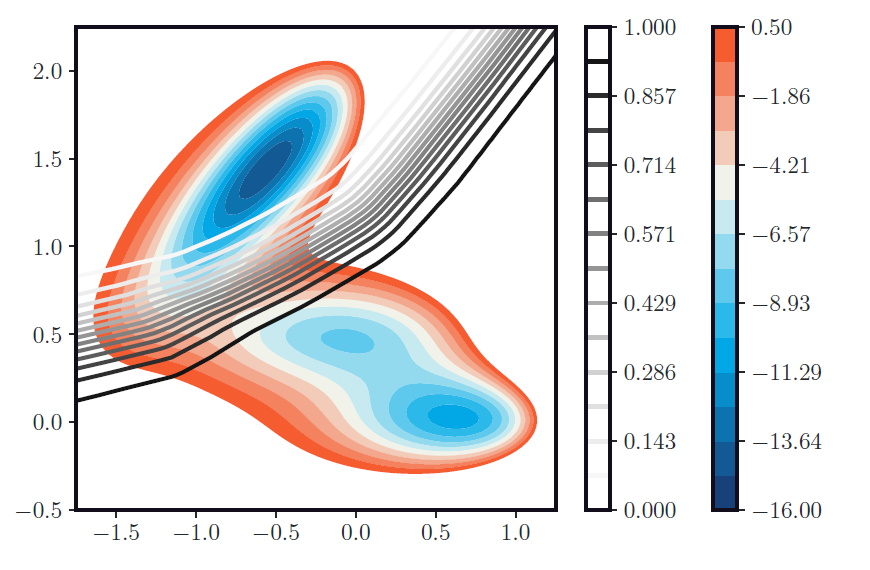
\includegraphics[width=0.7\linewidth]{./Figures/potential.png}
	\caption{Figure 1 from \textcite{rotskoff2020learning}: The potential function is shown as a contour plot. The isocommittor lines are shown from white to black. Notably, level set $q = 0.5$ coincides with the saddle, as expected.}
	\label{potential}
\end{figure}

We thus need to use an importance sampling technique; i.e., sample from another distribution and take into account this change of measure in the expectation computation. 
For more information on the importance sampling technique used see \textcite{thiede2016eigenvector}. 
Finally, the algorithm used in \textcite{rotskoff2020learning} is very similar with the one used in PINNs.
The difference lies in the points $\bx$ that the loss is evaluated on in each iteration of the algorithm. 
In the algorithm of \textcite{thiede2016eigenvector} for each iteration random locations are sampled according to a distribution that depends on both the potential $V(\bx)$ (the probability distribution) and the importance sampling functions.

%%%%%%%%%%%%%%%%%%%%%%%%%%%%%%%%%%%%%%%%%%%%%%%%%%%%%%%%%%%%%%%%%%%%%%%%%%%%%%%%%%%%%%%%%%%%%%%%%%%%%%%%%	

%\section*{Appendix}
\newpage	
\printbibliography[heading=bibintoc,title={References}]
	
\end{document}